\section{Introduction}
In this chapter, we revisit the fundamental stable marriage problem, which pertains to monogamous matchings of equinumerous male and female individuals. Specifically, we consider instances where each person's preference list comprises all members of the opposite sex, with strict preferences. In doing so, we aim to construct an algorithmically robust and informative representation of the complete set of stable matchings, as well as the corresponding marriage lattice $\mathcal{M}$, for this foundational problem.

\section{The Compact Representation}
\subsection{The Irreducible Stable Matching}
Let us consider a pair $(m, w) \in \mathcal{M}$, any matching containing $(m, w)$ is called an $(m,w)$\textit{-matching}, and we use $\mathcal{M}(m, w)$ to denote the set of all $(m, w)$\textit{-matchings} in $\mathcal{M}$. Note that, $\mathcal{M}(m, w)$ could be empty, but if $M$ and $M^\prime$ are matchings in $\mathcal{M}(m, w)$ then so are $M \vee M^\prime$ and $M \wedge M^\prime$ (From the previous chapter).

So $\mathcal{M}(m, w)$ forms a \textit{sublattice} of $\mathcal{M}$, and it follows that $\mathcal{M}(m, w)$ contains its own \textbf{man-optimal} matching, \textit{one that dominates all $(m, w)$-matchings}. Let us denote $M(m, w)$ to denote the unique man-optimal $(m, w)$\textit{-matching}.

A stable matching $\mathbf{M}$ will be called \textbf{irreducible} if $M$ is $M(m, w)$ for some $m$ and $w$. Let us use $I(\mathcal{M})$ to denote the \textit{set} of all irreducible stable matchings, and $(I(\mathcal{M}), \preceq)$ as the partial order on $I(\mathcal{M})$ under the dominance relation ($\preceq$) inherited from $M$.

\begin{figure}[ht]
  \centering
  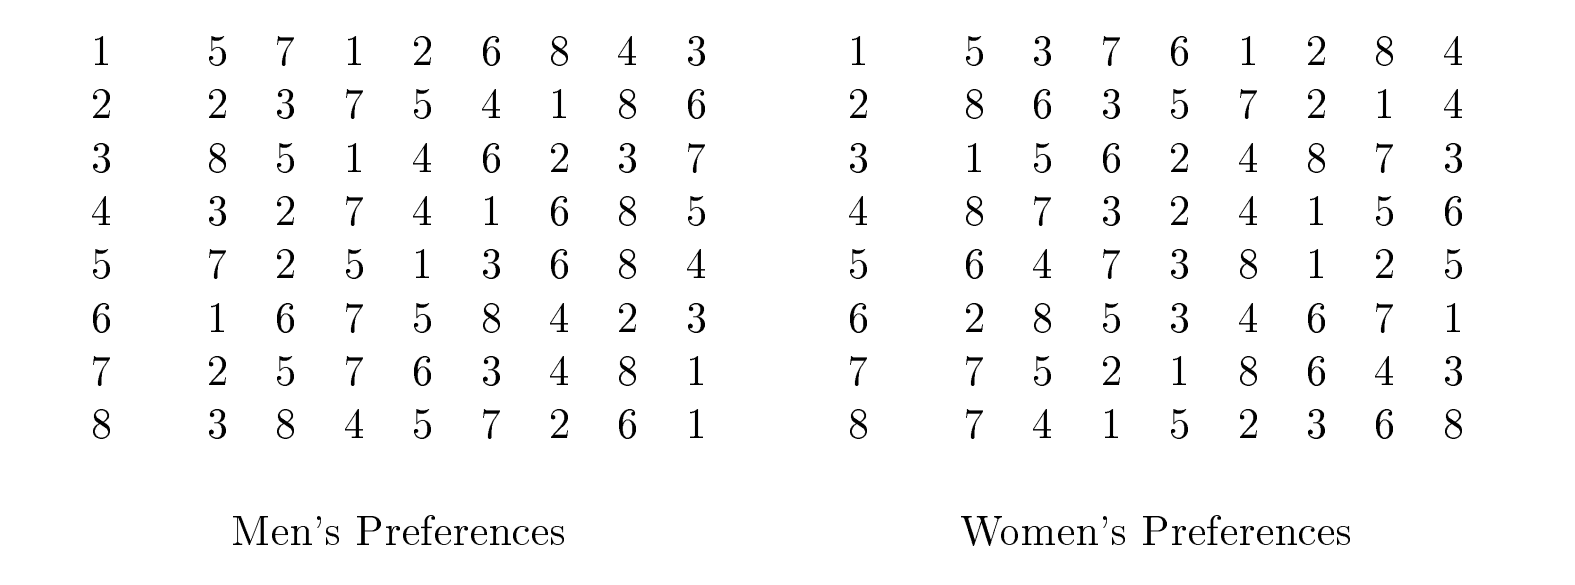
\includegraphics[width=1\textwidth]{IMAGES_FIGS/FIG_2_0.png}
  \caption{The stable marriage instance of size 8}
  \label{FIG_2_1}
\end{figure}

Let us consider the example of size eight. Here we have the lattice of 8 stable matchings for this instance. Each stable matching $M$ is described by a vector of length eight, where the number in position $i$ of the vector indicates the $M-partner$ of man $i$. Below each stable matching $M$ is a vector indicating the the ranking of the $M-partner$ of each man. 

\begin{figure}[ht]
  \centering
  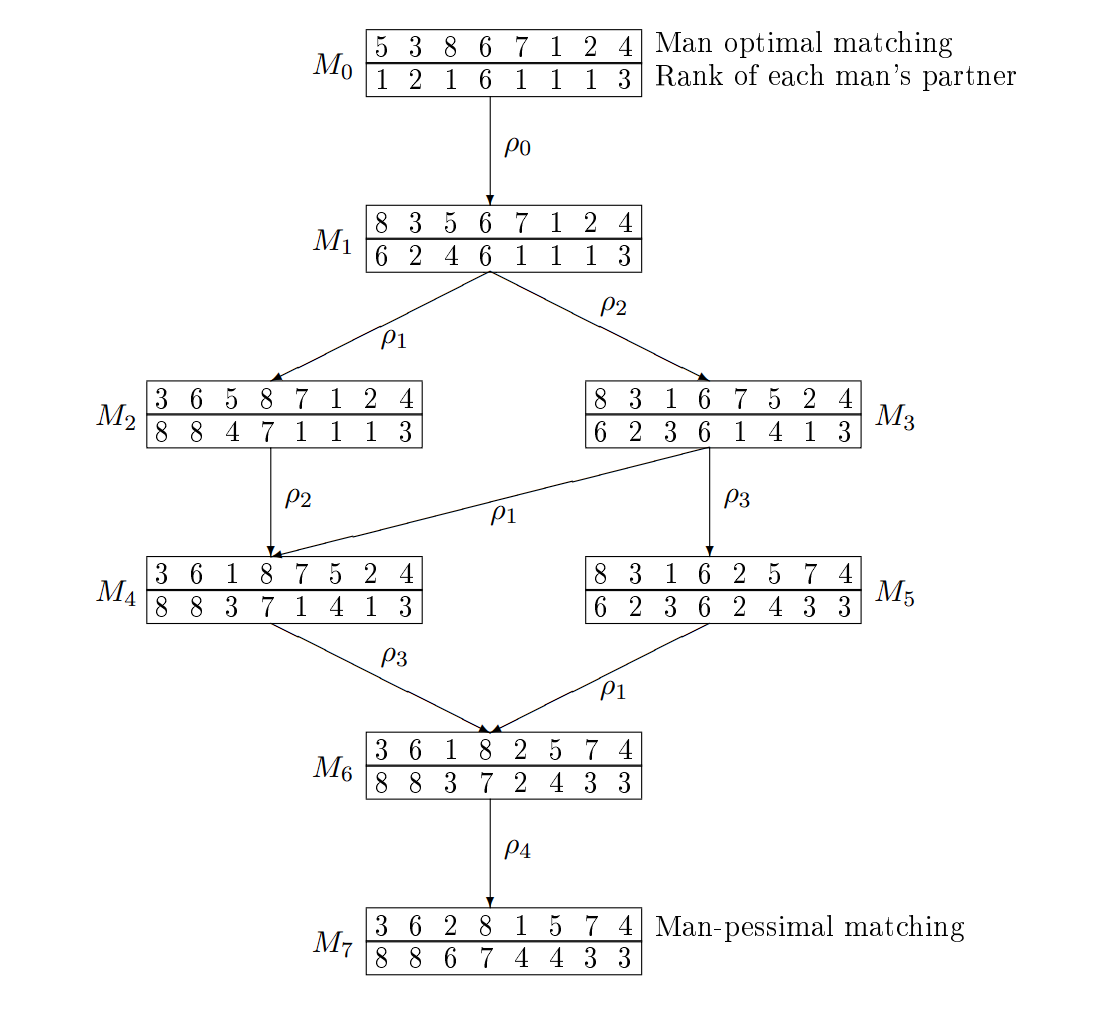
\includegraphics[width=0.9\textwidth]{IMAGES_FIGS/FIG_2_1.png}
  \caption{The lattice of stable matchings}
  \label{FIG_2_2}
\end{figure}

\begin{figure}[ht]
  \centering
  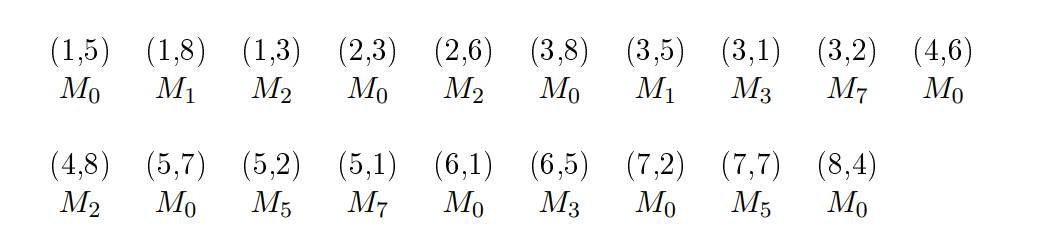
\includegraphics[width=0.8\textwidth]{IMAGES_FIGS/FIG_2_2.png}
  \caption{The stable pairs, and associated irreducible matchings}
  \label{FIG_2_3}
\end{figure}

\begin{figure}[ht]
  \centering
  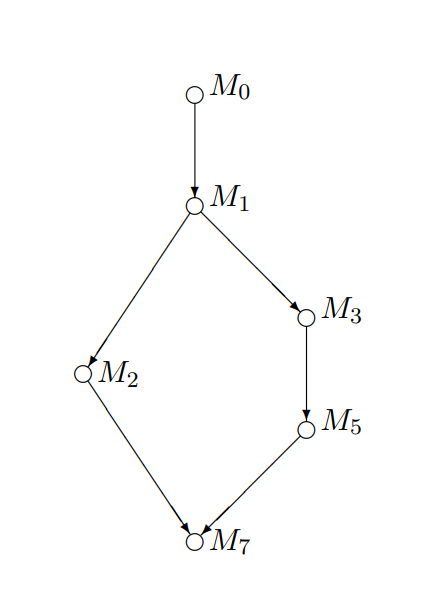
\includegraphics[width=0.4\textwidth]{IMAGES_FIGS/FIG_2_3.png}
  \caption{The partial order $I(\mathcal{M})$ for the irreducible stable matchings}
  \label{FIG_2_4}
\end{figure}

%make a box enclosing it
If $(R, \preceq)$ is a partial order, then a subset $S$ of $R$ is said to be \textbf{closed} in $R$ if there is no element in $R\backslash S$ that precedes an element in $S$.

A subset of matchings $S \subseteq M$ is closed in M if there is no matching in $M \\ S$ that dominates a matching in $S$.

Notice that, if $S$ is a subset of matchings in $I(\mathcal{M})$, then $\vee S$ is also a stable matching in $M$. Hence, every nonempty closed subset of $I(\mathcal{M})$ generates a stable matching in this way, and this defines a mapping from the nonempty closed subsets of $I(\mathcal{M})$ to $\mathcal{M}$. And we will show that this mapping is one-one.

For an arbitrary stable matching $M$, we define the irreducible support $U(M)$ of $M$ to be
$\{M(m, w) : (m, w) \in M\}$. 

\begin{exmp}\label{exmp_2_1}
    In the stable matchings of the above figure, the irreducible support of matching $M_3 = \{(1, 8),(2, 3),(3, 1),(4, 6),(5, 7),(6, 5),(7, 2),(8, 4)\}$ is $\{M_0, M_1, M_3\}$.
\end{exmp}

\begin{lemma}
\label{lem_2_1}
For any stable matching $M$, $M = \vee U(M)$.
\newline
\newline
\textit{{\small Any stable matching $M$ can be obtained by assigning each man to his least preferred partner among his partners in the matchings in $U(M)$}}
\end{lemma}

\begin{proof}
    Suppose $(m_1, w_1)$ is in $M$ but not in $\vee U(M)$. Since $(m_1, w_1)$ is in $M(m_1, w_1) \in U(M)$, there must be a pair $(m_2, w_2)$ in $M$ such that, in $M(m_2, w_2)$, man $m_1$ marries a woman strictly below $w_1$ in his list. Now $M(m_2, w_2)$ dominates all the stable matchings in which $m_2$ marries $w_2$, and in particular $M$. But this is a contradiction, because $m_1$ prefers $w_1$, his partner in $M$, to his partner in $M(m_2, w_2)$. Hence we have $M = \vee U(M)$.
\end{proof}

\begin{exmp}\label{exmp_2_2}
Woman $3$ is the worst partner for man $1$ among his partners in the matchings $\{M_0, M_2, M_3, M_5\} = U(M_6)$; woman $3$ is in fact the partner of man $1$ in $M_6$.
\end{exmp}

\begin{corollary}\label{cor_2_1}
Let $\hat{U}(M)$ be the set of all irreducible matchings that dominate some matching in $U(M)$. Then $M = \vee \hat{U}(M)$.
\end{corollary}

\begin{proof}
If a stable matching $M_1$ dominates stable matching $M_2$ then $M_1 \vee M_2 = M_2$, so $\vee \hat{U}(M) = \vee U(M)$, since each matching in $\hat{U}(M)$ dominates some matching in $U$.
\end{proof}

\begin{corollary}\label{cor_2_2}
A stable matching $M$ is $\vee S$ for a set $S$ of \textit{stable matchings} that excludes $M$, iff $M$ is not in $I(\mathcal{M})$
\end{corollary}

\begin{proof}
    The \textit{"if"} part follows from the Lemma studied earlier. Let's prove the converse part. First note that if $M = \vee S$, then every matching in $S$, dominates $M$. So if $M \notin S$, then for any pair $(m, w)$ in $M$ there is a matching $M^\prime$ in $S$ that contains $(m, w)$ and that strictly dominates $M$. So $M \neq M(m, w)$, and this is true for all pairs $(m, w)$ in $M$, so that $M$ cannot be in $I(\mathcal{M})$.
\end{proof}

Let's now prove that the mapping from the nonempty closed subsets of
$I(\mathcal{M})$ to $\mathcal{M}$ is one-one.

\begin{lemma}\label{lem_2_2}
    If $S$ and $T$ are \textit{distinct} closed subsets of $I(\mathcal{M})$, then $\vee S \neq \vee T$.
\end{lemma}

\begin{proof}
     Note, here that no maximal matching (with respect to dominance) of $S \cup T$ can dominate any other matching in $S \cup T$. Further, since $S \neq T$ and both subsets are closed in $I(\mathcal{M})$, one of the maximal matchings of $S \cup T$ cannot be in $S \cap T$. So one of the subsets, say $S$, contains a matching $M$ that does not dominate any matching in the other subset, $T$. Now $M = M(m, w)$ for some $m$ and $w$, so that $m$ has a partner no better than $w$ in $\vee S$. On the other hand, we claim that $m$ has a better partner than $w$ in every matching in $T$, so $\vee S$ cannot be $\vee T$. 
\end{proof}

\begin{theo}
So, in summary we have : 
\begin{itemize}
    \item There is a one-one correspondence between the nonempty closed subsets of $I(\mathcal{M})$ and the stable matchings of $\mathcal{M}$. This correspondence associates each stable matching $M$ with the irreducible stable matchings that dominates $M$.
    \item  If $S$ is the \textit{closed subset} of $I(\mathcal{M})$ corresponding to stable matching $M$, then $M = \vee S$.
    \item If closed subsets $S$ and $S^\prime$ of $I(\mathcal{M})$ correspond to matchings $M$ and $M^\prime$, respectively, then $M$ dominates $M^\prime$ \textbf{if and only if} $S \subseteq S^\prime$.
\end{itemize}

\end{theo}